\documentclass[10pt,twocolumn,letterpaper]{article}

\usepackage{cvpr}
\usepackage{times}
\usepackage{epsfig}
\usepackage{graphicx}
\usepackage{amsmath}
\usepackage{amssymb}
\usepackage{array}
\usepackage{xfrac}
\usepackage{amssymb}
%\usepackage{todonotes}
\usepackage{centernot}
\usepackage{textcomp}
\usepackage{blindtext}
\usepackage{centernot}
\usepackage{wasysym}
\usepackage{siunitx}
\usepackage[letterpaper]{geometry}
\usepackage{color}
%\usepackage[table]{xcolor}
\usepackage{amsfonts}
\usepackage{mathtools}
\usepackage{multirow}
\usepackage[small,it]{caption}
%\usepackage{titling}
%\usepackage{filecontents}
%\usepackage{titlesec}
\usepackage[section]{placeins}
%\usepackage[hidelinks]{hyperref}
%\usepackage{fancyhdr}
\usepackage{cancel}
%\usepackage{abstract}
\usepackage{minted}
\usepackage{widetext}
\usepackage[utf8]{inputenc}

\sisetup{output-exponent-marker=\textsc{e}}

\DeclareMathOperator*{\argmax}{arg\,max}
\DeclareMathOperator*{\argmin}{arg\,min}

\newcommand{\squishlist}{
 \begin{list}{$\bullet$}
  { \setlength{\itemsep}{0pt}
     \setlength{\parsep}{3pt}
     \setlength{\topsep}{3pt}
     \setlength{\partopsep}{0pt}
     \setlength{\leftmargin}{1.5em}
     \setlength{\labelwidth}{1em}
     \setlength{\labelsep}{0.5em} } }


\newcommand{\squishlisttwo}{
 \begin{list}{$\bullet$}
  { \setlength{\itemsep}{0pt}
    \setlength{\parsep}{0pt}
    \setlength{\topsep}{0pt}
    \setlength{\partopsep}{0pt}
    \setlength{\leftmargin}{2em}
    \setlength{\labelwidth}{1.5em}
    \setlength{\labelsep}{0.5em} } }

\newcommand{\squishend}{
  \end{list}  }
\footskip = 50pt
\setlength{\skip\footins}{10pt}

\newcommand*{\vertbar}{\rule[-1ex]{0.5pt}{3.0ex}}
\newcommand*{\horzbar}{\rule[.5ex]{2.5ex}{0.5pt}}

% Include other packages here, before hyperref.

% If you comment hyperref and then uncomment it, you should delete
% egpaper.aux before re-running latex.  (Or just hit 'q' on the first latex
% run, let it finish, and you should be clear).
\usepackage[breaklinks=true,bookmarks=false]{hyperref}

\cvprfinalcopy % *** Uncomment this line for the final submission

\def\cvprPaperID{****} % *** Enter the CVPR Paper ID here
\def\httilde{\mbox{\tt\raisebox{-.5ex}{\symbol{126}}}}

% Pages are numbered in submission mode, and unnumbered in camera-ready
%\ifcvprfinal\pagestyle{empty}\fi
\setcounter{page}{1}
\begin{document}

%%%%%%%%% TITLE
\title{Convolutional Neural Networks for texture classification}

\author{Edgar A. Margffoy-Tuay\\
Universidad de los Andes\\
201412566\\
{\tt\small ea.margffoy10@uniandes.edu.co}
% For a paper whose authors are all at the same institution,
% omit the following lines up until the closing ``}''.
% Additional authors and addresses can be added with ``\and'',
% just like the second author.
% To save space, use either the email address or home page, not both
%\and
%Second Author\\
%Institution2\\
%First line of institution2 address\\
%{\tt\small secondauthor@i2.org}
}

\maketitle
%\thispagestyle{empty}

%%%%%%%%% ABSTRACT
\begin{abstract}
We present a Convolutional Neural Network architecture suitable to classify texture images, our approach achieves a 90\% accuracy when evaluated over the validation set of Ponce's group texture dataset, compared with other classical approaches, such as Texton Dictionary representation, which achieves 60\% accuracy.
\end{abstract}

%Segmentation represents one of the core Computer Vision tasks in scientfic and academic research since the 1970s, this problem is defined as the grouping of pixels on a image according to several semantic categories of interest. Until recently, this problem was approached by using pixel-level mathematical formulations based on classical image processing and DSP, without any association with other Computer Vision problems nor any AI-related task, such as NLP. However, after the rise of

%%%%%%%%% BODY TEXT
\section{Introduction}
%\subsection*{Context}
Convolutional Neural Networks (CNN) were proposed by Yann LeCun \cite{Cun:1990:HDR:109230.109279} in 1988 to recognize digits. This class of specialized networks are based on a set of convolutional layers to compute a set of filters activations over an image input, which in turn are then aggregated via a set of Pooling layers. This architecture and layout allows to learn new features that cannot be described only by using a set of linear filters, such as the Texton Dictionary framework proposed by Malik et al on \cite{Malik2001}, on which, each image is represented by a Texton histogram dictionary computed from a set of activation responses between the image and a filter bank that contains different linear and blob detectors. 
\\
\\
In this framework, both approaches seem familiar, however, the main difference radicates in the filter initialization process, while a CNN starts with random filters which then are learned via backpropagation, the texton dictionary depends on a set of predefined filter bank. Also, the texton approach only considers first order filters, such as blob and edge detectors, while a CNN not only learns this first order filters, but it also learns more complex filters in latter layers, which improve the higher dimension representation of each image of the dataset. Finally, and more important is related to the classification representation vectors, while on the texton approach the representation relies on calculating K-Means over all the filter activations of an image, which then are given as an input to another classifier such as SVMs and Random Forests, a CNN allows to represent and classify at the same time, by using fully connected layers in the same fashion as a conventional Feed-Forward Neural Network, this allows to stack and propose several reference deep classification architectures, such as AlexNet \cite{Krizhevsky:2012:ICD:2999134.2999257}, VGG \cite{Simonyan14c}, ResNet \cite{he2016deep} and GoogLeNet \cite{szegedy2015going}, which achieved state-of-the-art performance on several classification challenges and benchmarks, such as ImageNet. 

\section{Materials and Methods}

\begin{figure*}[t]
	\centering
	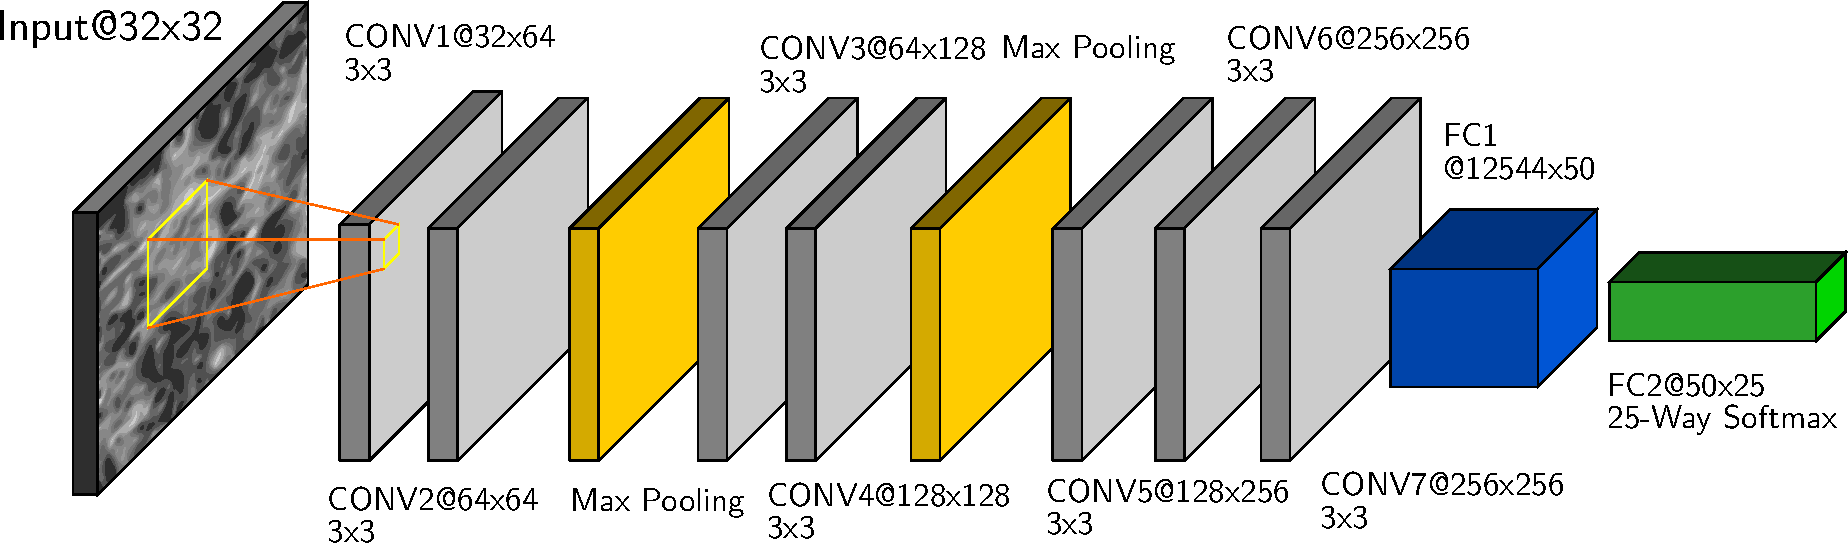
\epsfig{file=./Assets/EdNet.pdf,width=1.0\linewidth,clip=}
	\caption{Graphical description of the proposed convolutional neural network architecture}
	\label{Fig:F1}
\end{figure*}


The texture classification dataset consists of 1000 texture images of size 640$\times$480 grouped on 25 distinct categories, according to different light illumination conditions. Due to the reduced number of images present on the dataset, it is necessary to sample multiple texture patches of size 32$\times$32, this allows to increase the input image representation space, which should be suitable to train a CNN. 
\\
\\
The overall architecture consists of 7 convolutional stacked layers with kernel size $3\times3$ and stride of 1. The network is trained with a set of 2 fully connected layers that are mapped to a 25-way softmax layer. The non-linearity applied to all the convoltional and fully connected layers correspond to Rectified Linear Units (ReLu), which allow to discard all negative activations while not squashing the positive inputs to a single range. Max Pooling layers of size 2$\times$2 were defined twice between each pair of down-4 layers. The overall network architecture is presented on Figure~\ref{Fig:F1}.
\\
\\
The network was trained using random initialization during 100 epochs, the selected optimization method correspond to Stochastic Gradient Descent with momentum, the selected learning rate was fixed at \num{0.01}, and momentum rate of 0.5. To improve the convergence steps, the input set was normalized to have a mean of 0.485 and a variance of 0.229, this allows to unskew the error surface to a more convex form. Also, early stopping was used to prevent overfitting. Finally, the network implementation was done over PyTorch and trained using an NVIDIA Tesla K40 GPU.

%\begin{figure*}[t]
%	\centering
%	%	\begin{center}
%	%\fbox{\rule{0pt}{2in} \rule{0.9\linewidth}{0pt}}
%	\epsfig{file=./Assets/Model_red.pdf,width=0.8\linewidth,clip=}
%	%\includegraphics[width=0.8\linewidth]{egfigure.eps}
%	%	\end{center}
%	\caption{Visual description of the planned baseline to approach the image segmentation recovery problem given a video input. Images taken by the author}
%	\label{Fig:F1}
%	%\label{fig:long}
%	%\label{fig:onecol}
%\end{figure*}

%\begin{figure*}[t]
%	\centering
%	%	\begin{center}
%	%\fbox{\rule{0pt}{2in} \rule{0.9\linewidth}{0pt}}
%	\epsfig{file=./Assets/Model_red.pdf,width=0.8\linewidth,clip=}
%	%\includegraphics[width=0.8\linewidth]{egfigure.eps}
%	%	\end{center}
%	\caption{Visual description of the planned baseline to approach the image segmentation recovery problem given a video input. Images taken by the author}
%	\label{Fig:F1}
%	%\label{fig:long}
%	%\label{fig:onecol}
%\end{figure*}


\section{Results}
The network training architecture was modified several times to improve the weight adjustment without incurring in overfitting, initially, the network was proposed with a single Convolutional layer and a single connected layer. Under this model, the network was unable to achieve more than 24\% accuracy, this is due to the limitation of a single convolutional layer, which only allows to take an image and extract basic features based only on linear and blob filters, this approach is no different from taking a texture image and classify it via Texton Dictionary representation. To improve the accuracy, a total of four convolutional layers were stacked upon the first defined convolutional layer, this allowed to increase the accuracy of the model, from 24\%, up to 60\%. 
\\
\\
At this point it was necessary to test new training strategies, such as introducing pooling layers and also proabillistic Dropout, while dropout did not improve the accuracy of the model, adding pooling layers between each two stacked layers reduced the total number of convolutional actiavtions, and allowed to increase the total accuracy of model to 63\%, however, the total number of parameters trained did not explain and fit the texture data well. To further improve the model training, more convolutional layers were stacked, those layers help to correlate and explain better the lower convolutional features, while the lower convolutional layers help to learn basic features and filters, the upper layers allow to specialize the feature activations that adjust to single input cases.
\\
\\
After adding a set of three more convolutional layers, without any pooling layers, the accuracy increased to 90\% over the validation set and 98\% over the training set. As it can be shown on Table~\ref{Tab:Ablation}, the upper layers did improve the classification tasks, while more shallow networks do not perform well.

\begin{table}[H]
	\centering
	\begin{tabular}{|c|c|c|c|c|c|c|c|c|c|}
		\hline
		Network & Acc \\ \hline
		CONV1, FC1 & 24\% \\ \hline
		CONV1-4, FC1, FC2 & 60\% \\ \hline
		CONV1-4 (POOL), FC1, FC2 & 63\% \\ \hline
		CONV1-5 (POOL), FC1, FC2 & 70\% \\ \hline
		CONV1-6 (POOL), FC1, FC2 & 80\% \\ \hline
		CONV1-7 (POOL), FC1, FC2 & 90\% \\ \hline
	\end{tabular}
	\caption{Ablation tests done over the proposed neural network architecture}
	\label{Tab:Ablation}
\end{table}

\section{Conclusions}
Convolutional Neural Networks are suitable to large scale visual datasets, this model allows to represent an image by adding the responses of several filter layers that are learned via backpropagation, this approach allows to represent an input and classify it at the same time, without any distinction between feature representation and classifier, as it was the usual framework before 2012. 
\\
\\
Along the experiments proposed previously it was possible to analyse and identify the function of each of the stacked layers proposed, in each iteration it was possible to observe that adding more convolutional layers on top can help to improve the training convergence, however, this procedure must be controlled to reduce overfitting. 
\\
\\
With respect to the total number of layers present on the architecture, it is possible to conclude that the lower layers tend to be similar across all CNN domains, independent of the input dataset, this is due to the fact that these layers tend to learn simple features, such as linear filters, which are canonical for all CNN models, however, the difference between models are constrained by the top layer features, which are more expressive and specialized on the input dataset. This allows to finetune and refine the filter activation responses of a pretrained network over a larger dataset, such as ImageNet to adapt to new and unrelated datasets, with feasible and good results.
\\
\\
Finally, the number of Fully connected layers should be reduced should the model learns a sufficiently good set of features, which can be more expressive and simple than adding a more complex fully connected set of weights that increase both training space and time complexity.

{\small
\bibliographystyle{ieee}
\bibliography{egbib}
}


\newpage
%\section{Some Results}
%\begin{figure}[H]
%	\centering
%	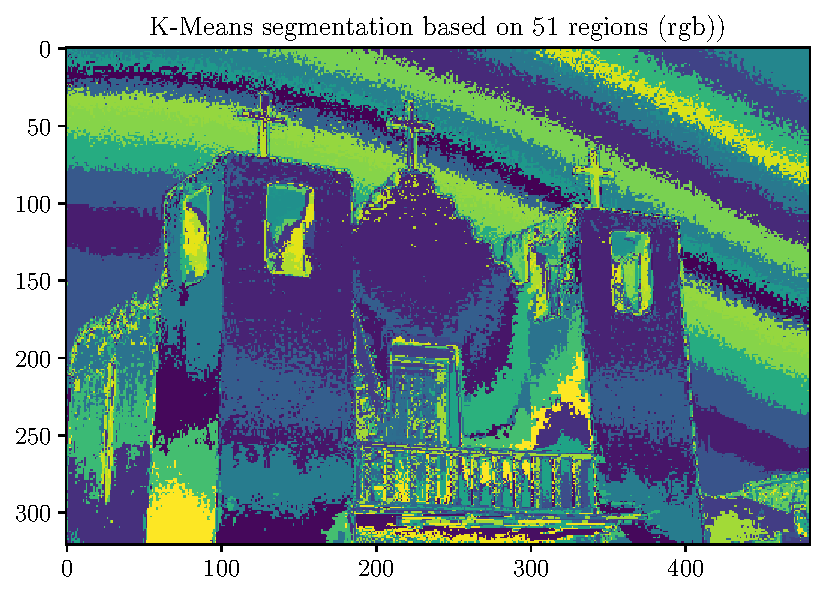
\epsfig{file=./Assets/24063_k-means_rgb_51.pdf,width=1.0\linewidth,clip=}
%	\caption{Example of K-Means segmentation result subject to 51 regions (No spatial)}
%	\label{Fig:kmeans1}
%\end{figure}
%
%
%\begin{figure}[H]
%	\centering
%	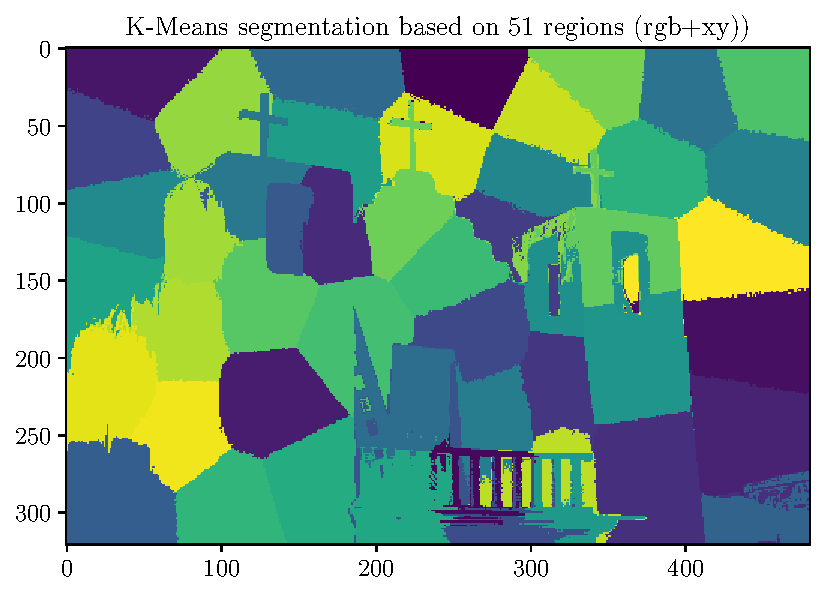
\epsfig{file=./Assets/24063_k-means_rgb+xy_51.pdf,width=1.0\linewidth,clip=}
%	\caption{Example of K-Means segmentation result subject to 51 regions (Spatial), this figure presents a large number of convex and spherical regions}
%	\label{Fig:kmeans2}
%\end{figure}
%
%\begin{figure}[H]
%	\centering
%	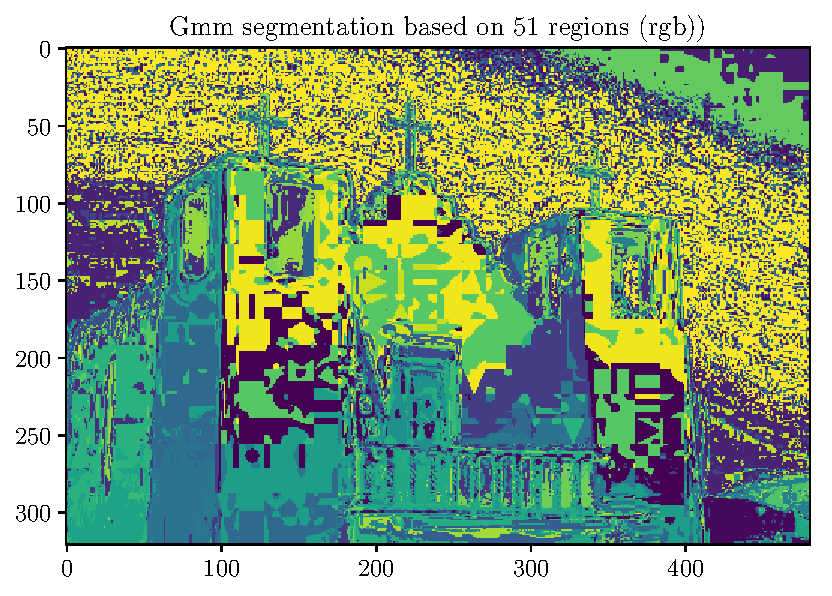
\epsfig{file=./Assets/24063_gmm_rgb_51.pdf,width=1.0\linewidth,clip=}
%	\caption{Example of GMM segmentation result subject to 51 regions (No spatial)}
%	\label{Fig:gmm1}
%\end{figure}
%
%\begin{figure}[H]
%	\centering
%	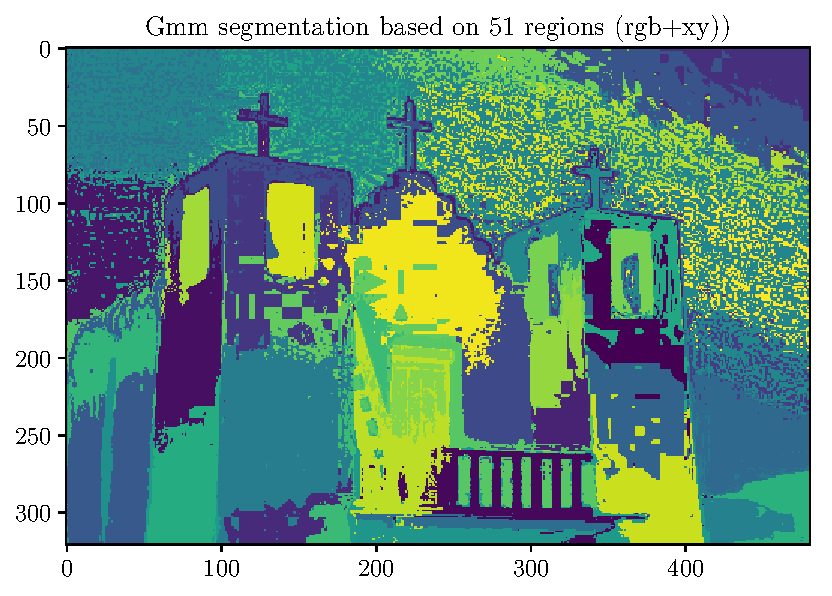
\epsfig{file=./Assets/24063_gmm_rgb+xy_51.pdf,width=1.0\linewidth,clip=}
%	\caption{Example of GMM segmentation result subject to 51 regions (Spatial information added), the noise was reduced}
%	\label{Fig:gmm2}
%\end{figure}
%
%\begin{figure}[H]
%	\centering
%	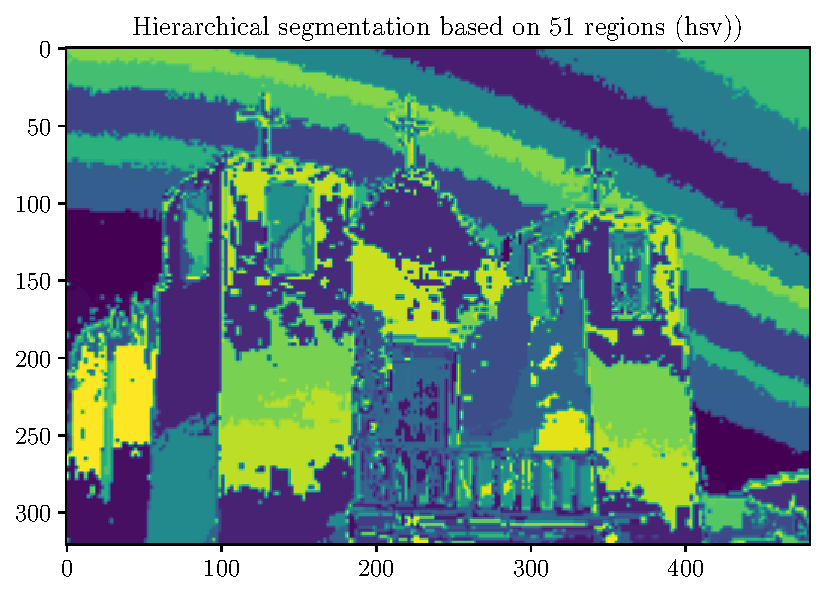
\epsfig{file=./Assets/24063_hierarchical_hsv_51.pdf,width=1.0\linewidth,clip=}
%	\caption{Example of Hierarchic segmentation result subject to 51 regions (No spatial information added), notice the smooth noise throughout all the regions by interpolation effects}
%	\label{Fig:hier1}
%\end{figure}
%
%\begin{figure}[H]
%	\centering
%	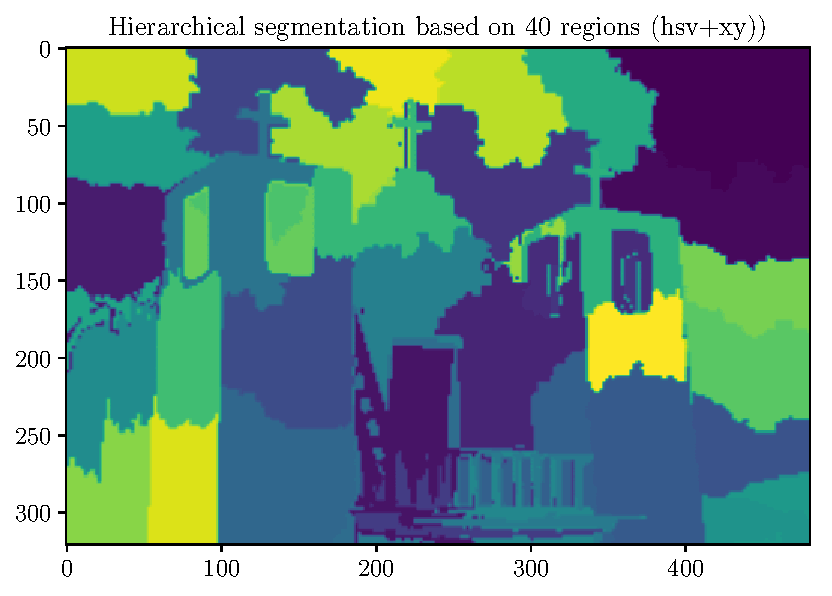
\epsfig{file=./Assets/24063_hierarchical_hsv+xy_40.pdf,width=1.0\linewidth,clip=}
%	\caption{Example of Hierarchic segmentation result subject to 40 regions (Spatial information added), notice the smooth noise throughout all the regions by interpolation effects}
%	\label{Fig:hier2}
%\end{figure}
%
%\begin{figure}[H]
%	\centering
%	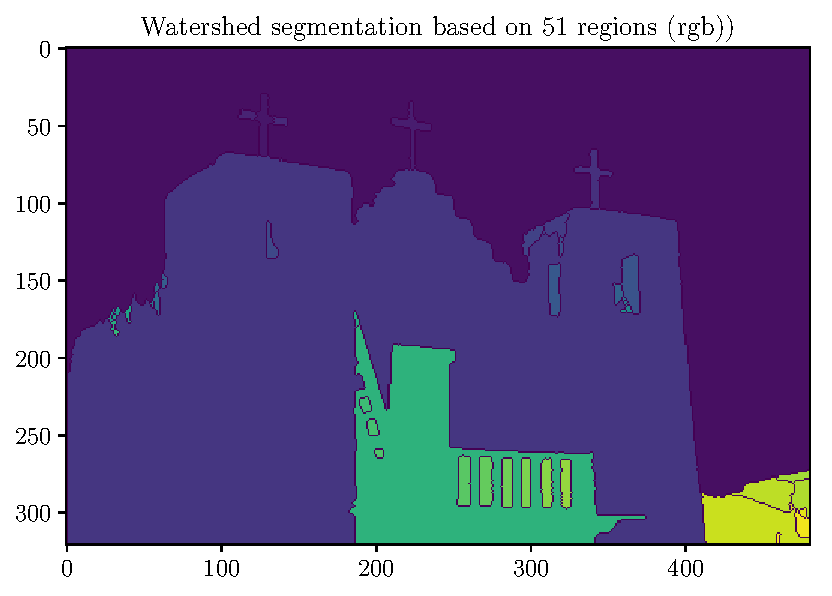
\epsfig{file=./Assets/24063_watershed_rgb_51.pdf,width=1.0\linewidth,clip=}
%	\caption{Example of H-Minima Watershed segmentation result subject to 51 regions, notice the well defined contours and regions}
%	\label{Fig:water1}
%\end{figure}
%
%\begin{figure}[H]
%	\centering
%	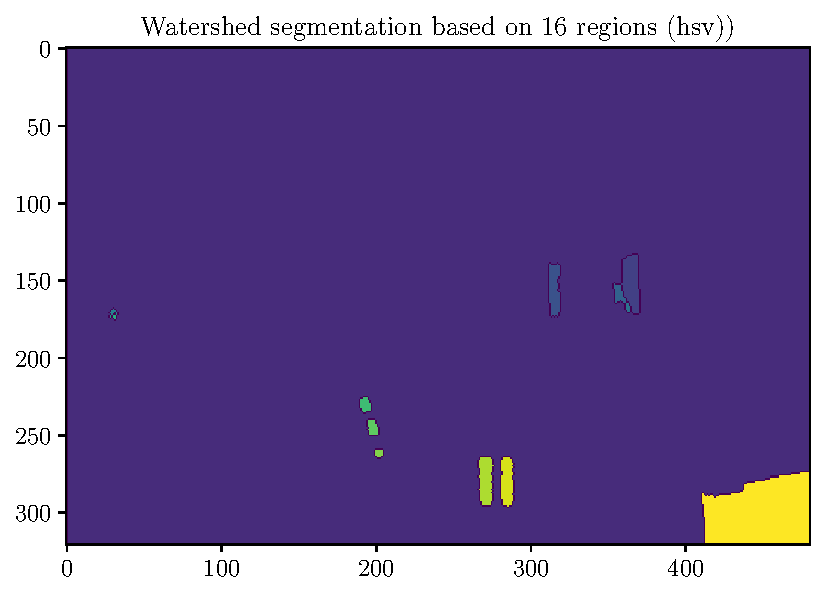
\epsfig{file=./Assets/24063_watershed_hsv_16.pdf,width=1.0\linewidth,clip=}
%	\caption{Example of H-Minima Watershed segmentation result subject to 16 regions, notice the disappearance of the main ROI}
%	\label{Fig:water2}
%\end{figure}



\end{document}
